\section{Auswertung}
\label{sec:Auswertung}

Die bei $\SI{0}{\milli\bar}$ gemessene Position des Maximums entspricht einer
Energie von ca. $\SI{4}{\MeV}$. Unter der Annahme einer linearen
Energieskala können mit diesem Startwert die anderen Energien $E_{\alpha}$
berechnet werden, die Ergebnisse sind in Tabelle \ref{tab:tab1} zu sehen.
Dort sind auch die nach Formel \ref{eqn:??} berechneten
effektiven Längen eingetragen, für die Berechneung wird der bei der
ersten Messung eingestelle Abstand von $x_0=\SI{2,5}{\cm}$ verwendet.

\begin{table}[H]
  \centering
  \caption{Messwerte der Wärmepumpe}
  \label{tab:tabe1}
    \begin{tabular}{S S S S S S}
    \toprule
    $ t  \: / \si{\second} $ & $ p_a \: / \si{\bar} $ & $ p_b \: / \si{\bar} $ &
    $ T_1 \: / \si{\kelvin} $ & $ T_2 \: / \si{\kelvin} $ & $ P \: / \: \si{\watt} $\\
    \midrule
    0 & 5.0 & 5.0 & 293.65 & 293.65 & 0 \\
    60 & 4.7 & 6.0 & 294.15 & 293.55 & 115 \\
    120 & 4.4 & 6.4 & 295.15 & 293.15 & 118 \\
    180 & 4.5 & 6.9 & 296.35 & 291.95 & 122 \\
    240 & 4.6 & 7.0 & 297.55 & 290.95 & 125 \\
    300 & 4.6 & 7.0 & 298.85 & 289.95 & 125 \\
    360 & 4.5 & 7.2 & 300.05 & 289.15 & 123 \\
    420 & 4.4 & 7.4 & 301.15 & 288.45 & 123 \\
    480 & 4.3 & 7.8 & 302.35 & 287.65 & 122 \\
    540 & 4.2 & 8.0 & 303.55 & 286.95 & 122 \\
    600 & 4.2 & 8.1 & 304.65 & 286.25 & 121 \\
    660 & 4.1 & 8.3 & 305.75 & 285.55 & 121 \\
    720 & 4.0 & 8.5 & 306.75 & 284.95 & 121 \\
    780 & 4.0 & 8.8 & 307.75 & 284.35 & 121 \\
    840 & 3.9 & 9.0 & 308.75 & 283.75 & 121 \\
    900 & 3.8 & 9.1 & 309.65 & 283.15 & 121 \\
    960 & 3.8 & 9.2 & 310.55 & 282.55 & 122 \\
    1020 & 3.8 & 9.5 & 311.45 & 282.05 & 122 \\
    1080 & 3.7 & 9.8 & 312.25 & 281.55 & 122 \\
    1140 & 3.7 & 10.0 & 313.05 & 281.15 & 122 \\
    1200 & 3.7 & 10.0 & 313.9 & 280.65 & 122 \\
    1260 & 3.6 & 10.2 & 314.65 & 280.25 & 123 \\
    1320 & 3.6 & 10.3 & 315.35 & 279.85 & 123 \\
    1380 & 3.6 & 10.6 & 316.15 & 279.45 & 124 \\
    1440 & 3.6 & 10.8 & 316.85 & 279.15 & 124 \\
    1500 & 3.6 & 11.0 & 317.55 & 278.75 & 124 \\
    1560 & 3.6 & 11.1 & 318.25 & 278.55 & 124 \\
    1620 & 3.6 & 11.2 & 318.95 & 278.25 & 125 \\
    1680 & 3.5 & 11.4 & 319.55 & 277.95 & 125 \\
    1740 & 3.5 & 11.5 & 320.15 & 277.65 & 125 \\
    1800 & 3.5 & 11.7 & 320.75 & 277.45 & 125 \\
    1860 & 3.5 & 11.9 & 321.35 & 277.25 & 125 \\
    1920 & 3.5 & 12.0 & 321.95 & 277.05 & 125 \\
    1980 & 3.5 & 12.1 & 322.45 & 276.95 & 125 \\








      \bottomrule
    \end{tabular}
\end{table}


Wird die Zählrate gegen die effektive Länge aufgetragen, so ergibt sich
Abbildung \ref{fig:plot1}.

\begin{figure}[H]
  \centering
  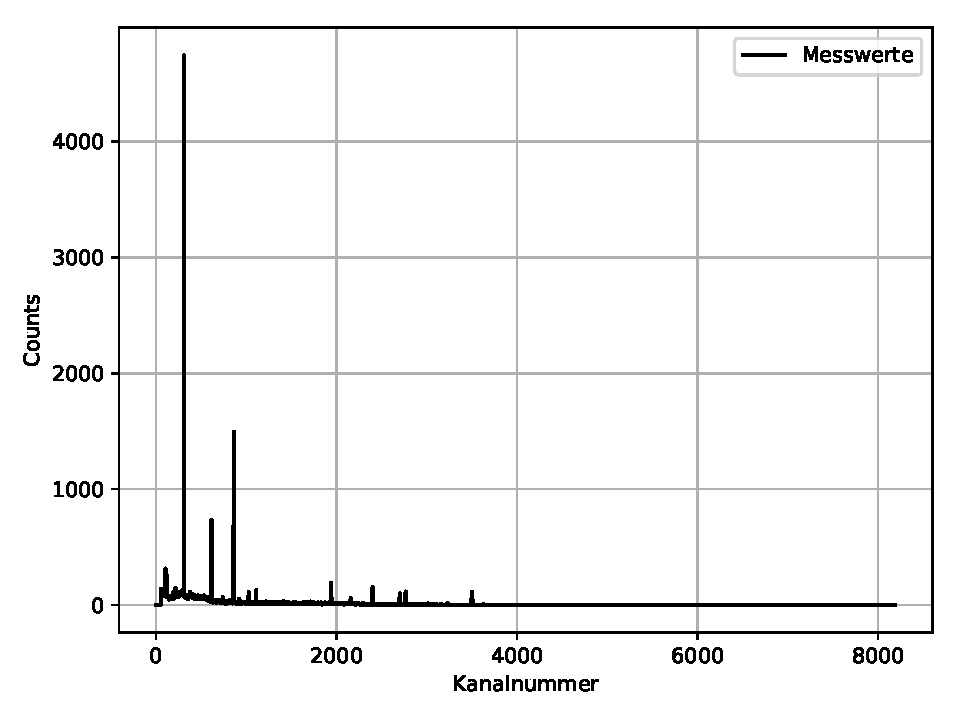
\includegraphics{plot1.pdf}
  \caption{}
  \label{fig:plot1}
\end{figure}

Die mittlere Reichweite der $\alpha$-Teilchen wird bestimmt, indem
der lineare Teil der Funktion gefittet wird, anschließend wird der
Geradenschnittpunkt mit $\sfrac{N}{2}$ gleichgesetzt. Durch umstellen
ergibt sich für die mittlere Reichweite die Formel:
\begin{equation}
  R_m=\frac{\sfrac{N}{2}-b}{m},
  \label{eqn:mittel}
\end{equation}
woraus sich die mittlere Reichweite von $\SI{1,93(23)}{\cm}$ ergibt.
Aus Gleichung \ref{eqn:??} ergibt sich somit eine Energie von
\begin{equation*}
  E_{\alpha}=\SI{0,122(29)}{\MeV}.
\end{equation*}

In Abbildung \ref{fig:plot2} wird die Energie gegen die effektive Länge aufgetragen,
aus der linearen Ausgleichsgeraden wird die Ableitung $\sfrac{dE}{dx}$ bestimmt, die
den Energieverlust $\sfrac{-dE}{dx}$ darstellt.
Es ergibt sich ein Energieverlust von:
\begin{equation*}
  \frac{-dE}{dx}=\SI{0,49(2)}{\MeV}.
\end{equation*}

Für die zweite Messreihe, dessen Messwerte in Tabelle \ref{tab:tab2} zu
sehen sind, wird ebenfalls die Zählrate $N$ gegen die effektive Länge $x$ aufgetragen.
An den Messwerten ist zu erkennen, das die Werte für die Zählrate deutlich langsamer
abfallen als das bei der ersten Messreihe der Fall ist.
Wie in Abbildung \ref{fig:plot2} zu sehen überschneiden sich die Messwerte nicht mit
der $\sfrac{N}{2}$-Linie. Daher kann die mittlere Reichweite und somit auch
die Energie nicht bestimmt werden.

\begin{figure}[H]
  \centering
  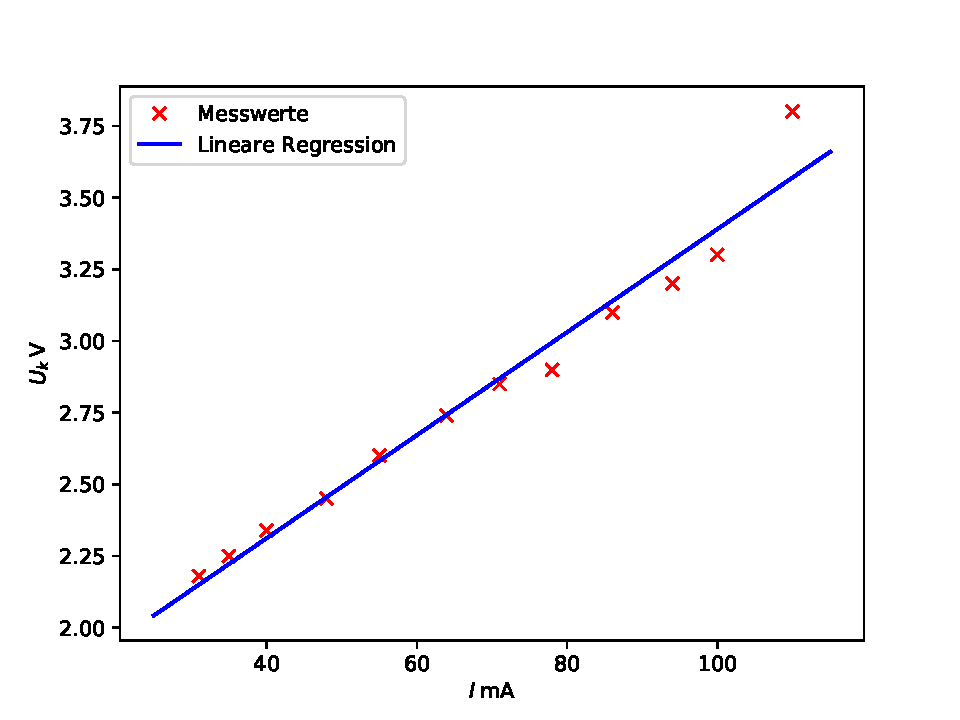
\includegraphics{plot2.pdf}
  \caption{}
  \label{fig:plot2}
\end{figure}


Die Messergebnisse des zweiten Versuchsteils sind in Tabelle \ref{tab:tab3}
dargestellt und werden in Abbildung \ref{fig:plot4} in einem Histogramm
veranschaulicht.

\begin{figure}[H]
  \centering
  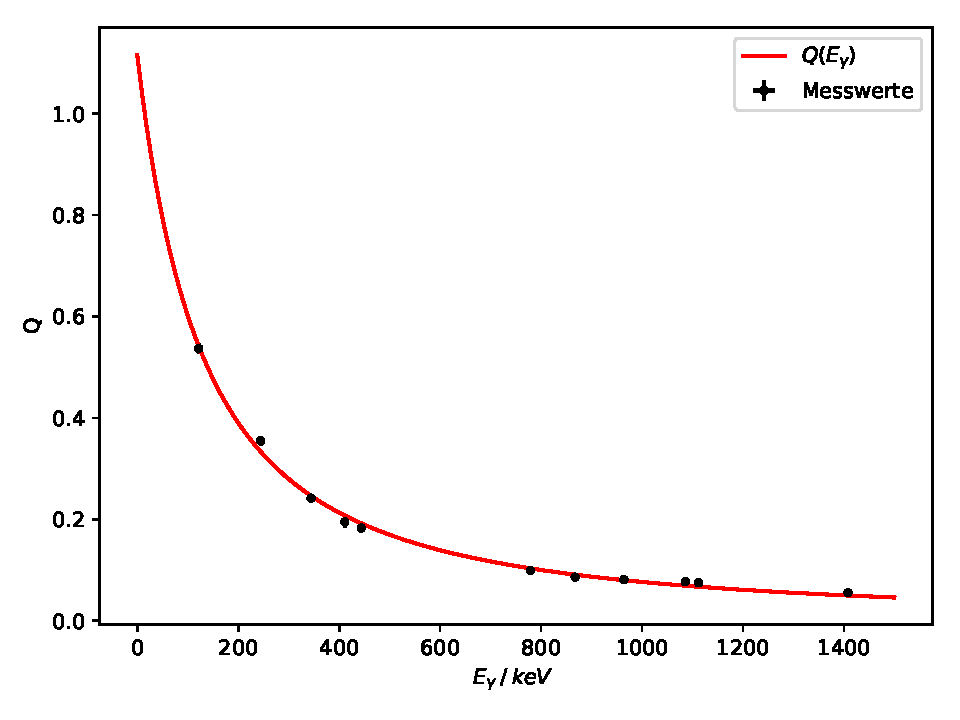
\includegraphics{plot4.pdf}
  \caption{}
  \label{fig:plot4}
\end{figure}

Es werden sowohl die Gauß-, als auch die Poissonverteilung eingezeichnet, um
diese mit den Messwerten vergleichen zu können.
Da die Poissonverteilung von dem Mittelwert der Messwerte und die
Gaußverteilung von dem Mittelwert $\bar{N}$ und der Varianz $\sigma^{2}$ abhängen werden diese ermittelt.
Dabei ist die VArianz das Quadrat der Standardabweichung $\sigma$.
\begin{align*}
  \bar{N}&=\SI{1015.52}{}\\
  \sigma^{2}&=\SI{10.88}{}\\
\end{align*}
